\section{Experiments}\label{s:exp}
Next, we present experimental results that suggest three main conclusions: (1) as a single framework, \sys can achieve parity in terms of accuracy with state-of-the-art approaches to a variety of different problems ranging from integrity constraint satisfaction, statistical data cleaning, and also data cleaning for machine learning, (2) it is possible to significantly reduce the runtime gap between \sys and specialized frameworks using simple pruning and distributed parallelization techniques, and (3) \sys enables automatic data cleaning for datasets containing a mixture of error types in an acceptable amount of time.  

\subsection{Datasets and Cleaning Tasks}
We list the main characteristics of the 8 experimental datasets, and describe them in more detail in our technical report~\cite{xxx}.

\stitle{Flight} The flight dataset~\cite{data-flights} contains arrival time, departure time, and gate information aggregated from 3 airline websites (AA, UA, Continental), 8 airport websites (e.g., SFO, DEN), and 27 third-party websites.
There are 1200 flight departures and arrivals at airline hubs recorded from each source.  Each flight has a unique and globally consistent ID, and the task is to reconcile data from different sources using the functional dependency \texttt{ID$\rightarrow$ arrival, departure, gate information}.

% The data cleaning problem is to reconcile the differences between each sources.  Each flight has a unique flight identifier that is consistent across the websites.  Formally, we can model the reconciliation problem as functional dependency between the flight id and the arrival time, departure time, gate information.  This enforces that after resolution there will be a single canonical version of those values.

\stitle{FEC} The election contributions dataset has 6,410,678 records, and 18 numerical, discrete, and text attributes. This dataset records the contribution amount and contributor demographic information e.g., name, address, and occupation.  The task is to enforce \texttt{city$\rightarrow$zipcode}, and match occupation to a codebook on canonical occupations.  The quality function is 1 if the occupation is in the codebook, and 0 otherwise; we penalize the edit distance between the original and edited occupation values.

% In this dataset, we enforced functional dependency relationships between city and zipcodes. We also matched the occupation of the contributors to a code book of popular occupations. This was posed as a quality function that was 1 only if the cell belonged to the code book and 0 otherwise, and there was an additive penalty on the edit distance between the change and the previous value.   


\stitle{Malasakit} This dataset contains 1493 survey disaster preparedness responses from the Philippines, with 15 numeric and discrete attributes. The task removes numerical outliers and remove dummy test records \ewu{Using XXX functional dependencies}.

\stitle{Physician} This dataset from Medicare.gov contains 37k US physican records, 10 attributes, with spelling errors in city names, zipcodes, and other text attributes. \ewu{What is the task and number of FDs}

\stitle{Census} This US adult census data contains 32k records, and 15 numeric and discrete attributes.  There are many missing values coded as 999999.  The task is to clean numeric values to build a classification model that predicts whether an adult earns more than $\$50k$ annually. 

\stitle{EEG}  The 2406 records are each a variable-length time-series of EEG readings (16 numeric attributes), and labeled as ``Preictal'' for pre-seizure and ``Interictal'' for non-seizure.  The goal is to predict seizures based on 32 features computed as the mean and avriance of the numeric EEG attributes.  The task is to identify and remove outlier reading values.  

% The training data is organized into ten minute EEG clips labeled "Preictal" for pre-seizure data segments, or "Interictal" for non-seizure data segments.  There are 2406 records each of which is a variable-length time-series of 16 attributes. We featurize this dataset into records of 32 attributes--the mean and variance over the length of the time-series.  This dataset primarily contains numerical outliers, the clips have spurious readings.

\stitle{Stock} There are 1000 ticker symbols from 55 sources for every trading day in a month~\cite{data-flights}.  The cleaning task involves (1) integrating the schemas by matching attributes across the sources (e.g., `prev. close' vs `Previous Close'), and then (2) reconciling daily ticker values values using primary-key-based functional dependencies akin to the flight dataset.

\stitle{Terrorism} The Global Terrorism Database~\cite{data-terrorism} is a dataset of around terrorist attacks scraped from news sources.  Each record contains the date, location, details about the attack, and the number of fatalities and injuries.  The dataset contains a mixture of data errors:
(1) there are many duplicates for the same terrorist incident,
(2) many missing values in the fatalities and injuries attributes are encoded as zeros, which overlaps with attacks that didnot have any fatalities/injuries, and
(3) the location attributes are inconsistently encoded.  
We used the dataset from 1970, and there are around $200$ records.  

We downloaded this dataset and sought to understand whether terrorist attacks have become more lethal than they were in the 1970s.  To do so, we hand cleaned the records to create a gold standard.  It turns out that, in this dataset, attacks have become more lethal, but fewer in number than 50 years ago.  This task was intentionally open-ended to represent the nature of the iterative analysis process.




% dataset considers data for 1000 ticker symbols from 55 sources that covers key trading metrics for every trading day in a month.  The challenge is to integrate the schema of these different sources. For example, in one source the closing price is denoted by 'Prev. Close' and in another it is 'Previous Close'.  Once the schema is consistent, there is a further data cleaning problem, where we would like to reconcile the values from different sources. This can be achieved with a similar functional dependency relationship as described for the flight datasets.  



\begin{figure}
    \centering
    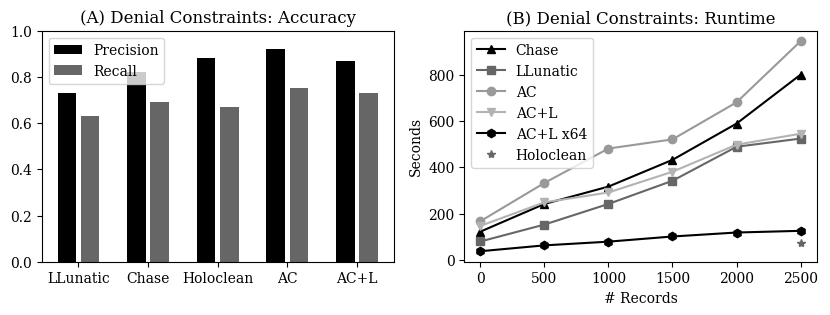
\includegraphics[width=\columnwidth]{exp/exp1.png}
    \caption{\small Comparison with denial constraint systems on the Flight dataset.  (A) \sys (AC) matches or exceeds the accuracy of the specialized systems.  (B) The structure of the data errors, along the learning and parallelization (AC+L x64) lets \sys scale sub-linearly and outperform all but HoloClean's reported runtimes.  \label{exp1a}}
\end{figure}

\subsection{Comparisons with Specialized Cleaning}
This subsection compares \sys to specialized cleaning approaches.  We illustrate that \sys can achieve comparable or higher accuracy, and the trade-offs in its runtime performance as compared to the baselines.

\subsubsection{Denial Constraints}
Denial constraints express a wide range of integrity constraints and form the basis of many data cleaning systems~\cite{llunatic,chase,holoclean}.  Although \sys may not fully enforce integrity constraints, we can compose a quality function can quantifies the number of constraint violations and find transformation that reduce the number of violations.    We use the Flight dataset for these experiments.

% Several data cleaning systems use Denial Constraints for constraint specification.  While \sys does not enforce integrity constraints, we can create a data quality objective function that quantifies the number of unsatisfied constraints.  This will search over a set of transformations that maximally satisfy these constraints.

\stitle{Baselines} We run against (1) Llunatic, a denial constraint-based cleaning system~\cite{DBLP:conf/sigmod/DallachiesaEEEIOT13} implemented in C++ on top of PostgreSQL, and (2) a restricted chase algorithm~\cite{benedikt2017benchmarking} implemented in Python. We compare against the chase because a large portion of denial constraints are functional dependencies~\cite{}, and can be resolved using fixed-point iteration.  We report numbers from the recent Holoclean publication~\cite{rekatsinas2017holoclean} that used the same datasets and constraints, but did not run the experiment ourselves.

\stitle{Results: } Figure \ref{exp1a}a shows the precision and recall of each approaches based on known ground truth. \sys matches or beats the accuracy of the baselines, however its runtime (AC) without any learning scales poorly compared to alternatives (\Cref{exp1b}b).  Using learning (AC+L) shows performance on par with LLunatic, and parallelization on 64 threads is comparable to Holoclean's reported runtime. The results suggest that learning exhibits sublinear scaling due to \sys learning more effective pruning rules as it sees more data.  These performance gains are at the expense of slightly reduced accuracy. 

We also evaluated \sys (single threaded, without learning) on the FEC, Malasakit, and Physician datasets.  Their precision, recall, and runtimes are as follows: 
FEC: $94\%$ prec, $68\%$ rec, $5$hrs; 
Malasakit: $100\%$ prec, $85\%$ rec, $0.39$hrs;
Physician: $100\%$ prec, $84\%$, $3.4$hrs.

% \begin{table}[ht]
% \footnotesize
% \small
% \centering
% \begin{tabular}{|l|r|r|r|r|r|r|r|}
% \hline
%  & \#rows & \#cols & Precision & Recall & Runtime \\
% \hline
% \hline
% FEC	&6M&18&0.94&	0.68&	5hrs\\
% \hline
% Malasakit &1493& 15& 1.0 & 0.85& 0.39hrs\\
% \hline
% Physican	&37k&10&1.0&0.84& 3.2hrs\\
% \hline
% \end{tabular}
% \end{table}

\begin{figure}
    \centering
    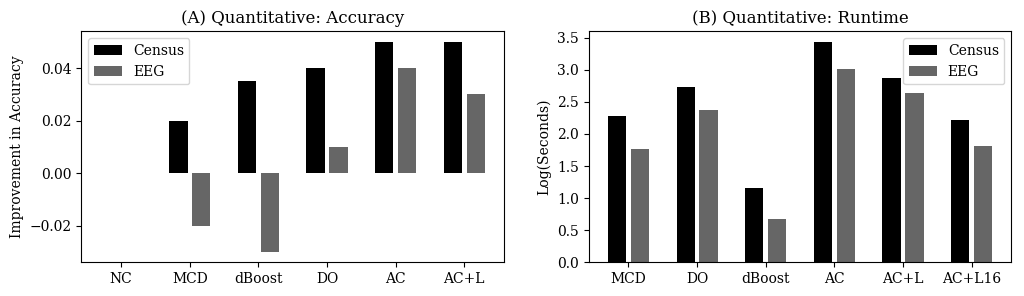
\includegraphics[width=\columnwidth]{exp/exp2.png}
    \caption{\small Quantitative data cleaning on census and EEG datasets for a classification application.  \sys tranformation can clip outliers or set them to a default value. (A) \sys ha higher accuracy than outlier detection algorithms (MCD, dBoost), and \sys with a single transform template (DO).  (B) Optimizations improve \sys runtime by over an order of magnitude.  \label{exp2a}}
\end{figure}

\subsubsection{Quantitative Data Cleaning}\label{s:expquant}
This experiment performs numerical cleaning on machine learning data.  In these applications, prediction labels and test records are typically clean and available (e.g., results of a sales lead), whereas the training features are often integrated from disparate sources and exhibit considerable noise (e.g., outliers).  Our quality function is simply defined as the model's accuracy on a training hold-out set, and we report the test accuracy on a separate test set.

We trained a binary classification random forest model using \texttt{sklearn} on the Census and EEG datasets.  We used standard featurizers (hot-one encoding for categorical data, bag-of-words for string data, numerical data as is) similar to~\cite{gokhale2014corleone}. 
\ewu{We split the dataset into 20\% test and 80\% training, and further split training into 20/80 into hold-out and training.  We run the search over the training data, and evaluate the quality function using the hold-out.  Final numbers are reported using the test data.  }


% The quality function for \sys is 0 for each record that is incorrectly predicted by the model, 1 for each record that is correctly predicted by the model.


% In many machine learning settings, cleanly labeled test data is often available (e.g., the results of following a sales lead). 
% Labels often represent directly observed phenomena making them relatively clean, while features are often weaker signals integrated from multiple disparate sources and subject to error and frequent change.
% This allows us to define a quality function in terms of the model's predictive accuracy--the data cleaning being a means to improving that predictive accuracy.

We defined the following three data transformation templates that sets numerical attribute values in $R$ if they satsify a predicate:

{\small
\begin{itemize}[leftmargin=*, topsep=0mm, itemsep=0mm]
  \item \stitle{\textsf{clip\_gt(attr, thresh)}} $R.attr = thresh$ if $R.attr>thresh$
  \item \stitle{\textsf{clip\_lt(attr, thresh)}} $R.attr = thresh$ if $R.attr<thresh$
  \item \stitle{\textsf{default(attr, badval)}} $R.attr$ set to mean val if $R.attr=badval$
\end{itemize}
}

\stitle{Baselines} We compare with 4 baselines: {\it No Cleaning (NC)}, {\it Minimum Covariance Determinant (MCD)} is a robust outlier detection algorithm used in~\cite{bailis2016macrobase} and sets all detected outliers to the mean value, {\it dBoost} uses a fast partitioned histogram technique to detect outliers~\cite{mariet2016outlier}, and {\it Default Only (DO)} runs \sys with only the \textsf{default()} transformation.  

\stitle{Results} The classifer achieves 82\% and 79\% accuracy on the uncleaned census and EEG data, respectively.  Most outliers in the census data are far from the mean, so MCD and dBoost can effectively find.  Further, setting census outliers to the mean is sensible. However, the same fix is not appropriate for the EEG data; it is better to clip the outlier values, thus MCD, dBoost, and DO have negligible or negative impact on accuracy.  When we realized this from running DO, it was straightforward to add the clipping transformations to the language, and with no other changes, re-run \sys with drastically improved EEG accuracies.  

Vanilla \sys (AC) is nearly $10\times$ slower than MCD, but the adding learning and 16-thread parallelization  matches MCD's runtimes.  dBoost is specialized for fast outlier detection and \sys is unlikely to match its runtime.  


\begin{figure}
    \centering
    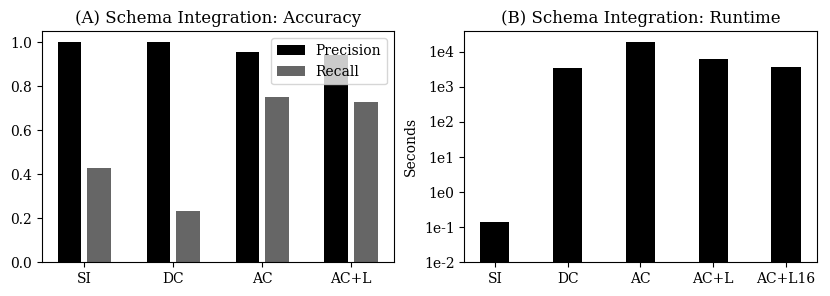
\includegraphics[width=\columnwidth]{exp/exp3.png}
    \caption{\small Schema integration and functional dependency errors in the stock dataset.  Cleaning schema integration (SI) or functional dependencies (DC) in isolation results in high precision but poor recall.  \sys cleans both types of errors with higher recall, and is as fast as DC.  \label{exp3a}}
\end{figure}

\begin{figure}[ht]
    \centering
    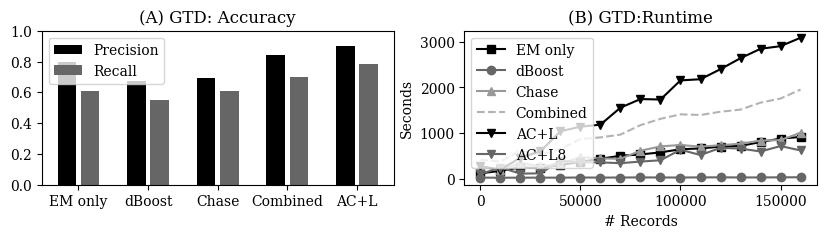
\includegraphics[width=\columnwidth]{exp/exp7.png}
    \caption{The Global Terrorism Database is a dataset of terrorist attacks scraped from news sources since 1970. (A) Shows that \sys can integrate many different forms of cleaning that were previously handled by disparate systems, (B) \sys achieves a competitive runtime to using all of the different system and accounting for data transfer time between them. \label{exp7a}}
\end{figure}

\subsubsection{Schema Integration}
We now evaluate cleaning on the stock dataset~\cite{data-flights} from 55 different sources that contains a mixture of schema integration and functional dependency errors.

\vspace{0.5em}\noindent\textbf{Baselines: } We compare approaches for each error type in isolation.  Schema Integration  (SI) matches attributes based on attribute name string similarity, and Data Cleaning (DC) assumes schemas are consistent and enforces functions dependencies using a restricted chase~\cite{benedikt2017benchmarking}.

\vspace{0.5em}\noindent\textbf{Results: } The specialized cleaning approaches exhibit high precision but low recall, as they miss records with multiple errors (\Cref{exp3a}).  \sys can mix both tasks in the quality function and has comparable precision with much higher recall.  SI is significantly faster since it only reads schema metadata, however \sys with learning and 16 threads is competitive with DC.  
\begin{figure*}[ht]
\centering
 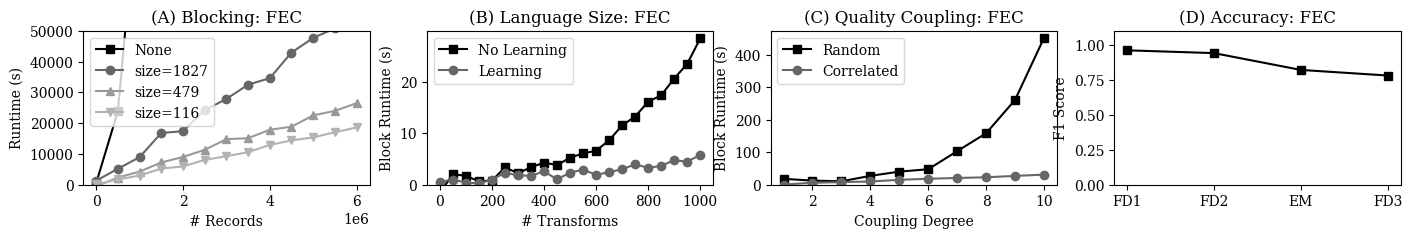
\includegraphics[width=\textwidth]{exp/exp4.png}
 \caption{\small (A) The degree of block-wise partitioning directly affects search time, (B) increasing the transformation language $\Sigma$ exponentially increases the search time, but learning is very effective at pruning the increased search space, (C) quality functions that couple errors between random records are significantly harder to optimize, (D) \sys degrades gracefully when adding irrelevant error types to the problem.  
 \label{fig:microbenchmarks}}
\end{figure*}

\subsection{Mixing Error Classes}
In the next experiment, we use the Terrorism dataset~\cite{data-terrorism} to evaluate \sys's support of multiple error classes.  

\stitle{Baselines} We hand-coded an entity matching (EM) algorithm that uses blocking to handle duplicate records.  We modeled the missing values as an outlier cleaning problem and used the dBoost~\cite{} library (dBoost). We modeled the location inconsistencies as a functional dependency problem and implemented a restricted chase algorithm (Chase).  Finally, we ran EM, dBoost, and Chase serially on the dataset (Combined).

\stitle{Results} \Cref{exp7a}a shows that combining and cleaning all three classes of errors within the same \sys framework (AC) achieves higher precision and recall than all baselines.  \ewu{In fact, the combined baselines still does not achieve \sys's level of accuracy because the cleaning operations need to be interleaved differently for different blocks.}   Although \sys is slower than any individual baseline, parallelizing \sys to \ewu{XXX} threads is faster than the combined baseline by \ewu{FOO$\times$}. 


% Error type (1) is best handled with a blocking and matching entity matching approach. Error type (2) is best handled with an outlier detector, where outliers are replaced with null values. Error type (3) is best addressed by a Functional Dependency.
% Figure \ref{exp7a}a shows how each individual system is not sufficient to clean the data.
% For (1) and (3), we coded a specialized algorithm in Python to address those errors.
% For (2), we used the dBoost library.
% \sys can model all of these in a single framework and can get the best combined performance.
% \sys achieves the highest precision and recall.
% \sys also achieves a competitive runtime to using all of the different system and accounting for data transfer time between them.


\begin{figure}
    \centering
    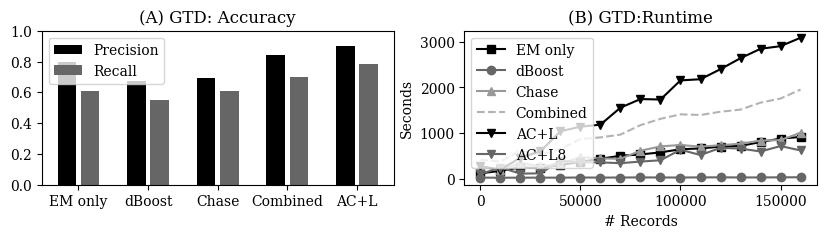
\includegraphics[width=\columnwidth]{exp/exp7.png}
    \caption{\small The terrorism dataset contains 3 classe of errors. (A) A unified cleaning framework outperforms individual cleaning approaches and even a serial combination.  (B) \sys is easily parallelized to \ewu{XXX} threads to outperform the combined baselines.  \label{exp7a}}
\end{figure}

\subsection{\sys In Depth}
This subsection uses the FEC setup to study the parameters that affect \sys's accuracy and runtime, the robustness of its cleaning programs, and its algorithmic properties.

\subsubsection{Algorithmic Sensitivity}

\stitle{Block-wise Cleaning} Partitioning the dataset into smaller blocks effectively reduces the problem complexity.  This can have tremendous performance benefits when each block exhibits very few errors that are independent of the other blocks.  \Cref{fig:microbenchmarks}a shows the performance benefits when varying the block size; we define the blocks by partitioning on three different attributes that have different domain sizes.  Reducing the block size directly improves the runtime; the search is effectively non-terminating when blocking is not used.    

\stitle{Language} \Cref{fig:microbenchmarks}b fixes the input to a single block, and evaluates the runtime based on the size of the language $|\Sigma|$.  Increasing the transformations increases the branching factor of the search problem. The search time is exponential in the language, however \sys's learning optimization can identify a pruning model that reduces the runtime to linear.

\stitle{Coupling in the Quality Function} The complexity of the quality function directly affects search time.  A cell-separable quality function is the simplest to optimize because each cell in the relation can be analyzed and cleaned in isolation.  In contrast, a quality function that couples multiple records together is more challenging to optimize because a longer sequence of transformation may be needed to sufficiently clean the records and improve the quality function.  

We evaluate this by artificially coupling between 1-10 records together, and creating a quality function that only improves when an attribute of the coupled records all have the same value.  We perform this coupling in two ways: {\it Random} couples randomly selected records, whereas {\it Correlated} first sorts the relation an attribute and couple records within a continuous range.  We expect that the random coupling requires individual cleaning operations for each record based on their IDs, whereas the correlated setting both allows \sys to exploit the correlated structure to learn effective pruning rules and \ewu{to clean the coupled records using a single cleaning operation}.  \Cref{fig:microbenchmarks}c shows that this is indeed the case when running \sys on a single fixed-size block. {\it Random} slows down exponentially with increased coupling, whereas {\it Correlated} increases linearly.

% The nature of the quality function also affects the search time. Quality functions that couple multiple records together are harder to optimize (Figure \ref{fig:microbenchmarks}c).
% Consider a function that requires that two different records must have the same attribute values.
% More transformations have to be achieved in a particular sequence before an improvement in quality is observed. 
% We selected between 1-10 records at random in each block and created a quality function that coupled these records together.
% As the degree of coupling increases, the search time grows quite drastically.
% We repeated the same experiment where now coupling is correlated with the data, i.e., we sort one of the attributes and couple ``nearby'' records.
% \sys performs significantly better on this version of the task.
% This is due to the learned pruning in \sys.
% Sorting the attributes introduces a systematic correlation in the quality function.
% \sys quickly learns a model which learns this correlation and uses that to prune the search space.

\stitle{Quality Function Complexity} Finally, we incrementally increase the quality function's complexity and show haw it affects the cleaning accuracy.  We add the following constraints in sequence: one functional dependency (FD), a second FD, an entity resolution similarity rule, and a third FD.  We define the quality function as the sum of each constraint's quality function.   \Cref{fig:microbenchmarks}d shows that the F1 accuracy decreases as more constraints are added, however the F1 score is still above $75\%$.  


 \begin{figure*}[ht]
\centering
 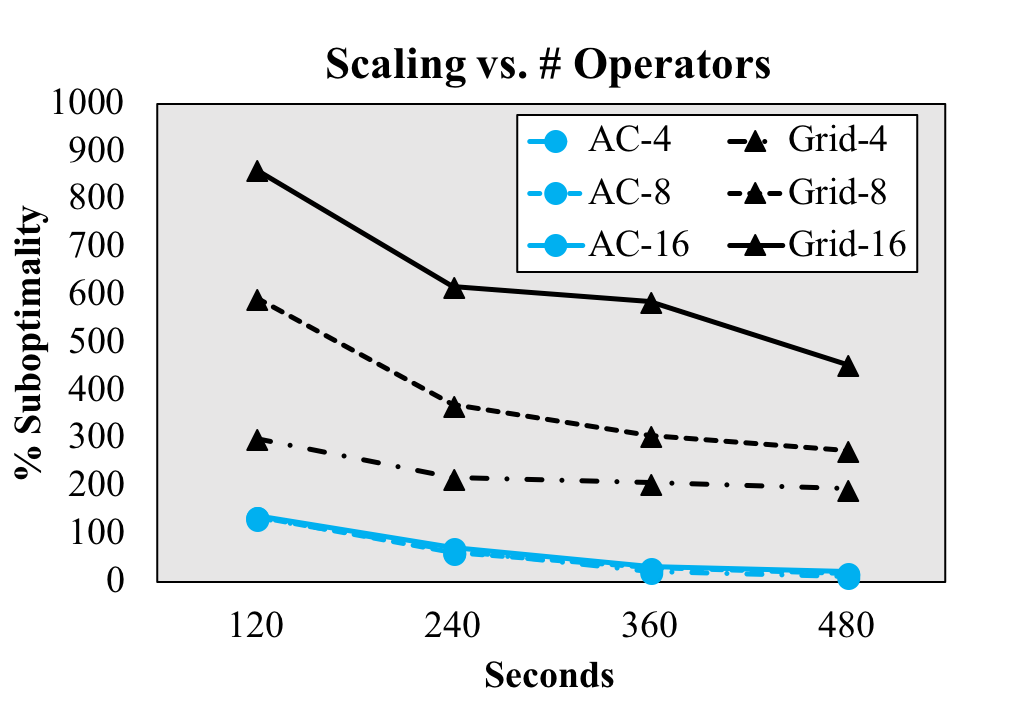
\includegraphics[width=\textwidth]{exp/exp5.png}
 \caption{\small (A) Regularization by increasing an editCost penalty makes \sys more robust to noisy (mis-specified) quality functions, (B-C) overly expressive transformation templates can lead to overfitting (2 attr) or an infeasibly large search space (3 attr).  
 \label{fig:sensitivity}}
\end{figure*}

\subsubsection{Cleaning Generalization and Overfitting}
An important characteristic of generating cleaning solutions as {\it programs} is that we can evaluate the program's robustness in terms of machine learning concepts such as overfitting and generalization.    To this end, we examine two concepts in the context of data cleaning: regularizaton and overfitting.  We also find that \sys's high level interface is helpful for iteratively tuning the cleaning process.

\stitle{Regularization}  Misspecified quality functions can cause \sys to output poorly performing cleaning programs.  We simulate this by adding random noise to the output of the quality function. \Cref{fig:sensitivity}A plots the F1-score of \sys on the FEC experiment while varying the amount of noise.  As expected, the output program's F1-score rapidly degrades as the noise increases.  

Machine learning uses regularizing penalty terms to prevent overfitting.  We can similarly add a penalty to the quality function to prevent too many edits.  Each line line shows the edit cost penalty and shows that although the F1 is lower when there is no noise, \sys is more robust to larger amounts of noise. 

\stitle{Overfitting} In machine learning, over-parameterized models may be susceptible to overfitting.  A similar property is possible if the language $\Sigma$ is overly expressive.  We use a transformation template that finds records matching a parameterized predicate and sets an attribute to another value in its instance domain.   We then vary the language expressiveness by increasing number of attributes in the predicate between 1 and 3.  Finally, we run \sys on a training sample of the dataset (x-axis), and report F1 accuracy on the training and a separate test sample (\Cref{fig:sensitivity}B-C).  Note that overfitting occurs when the training accuracy is significantly higher than test accuracy.

Indeed we find an interesting trade-off.  The 1 attribute predicate performed worst on the training sample but outperformed the alternatives on the test sample.  The 2 attribute predicate was more expressive and overfit to the training data.  Finally, the 3 attribute predicate is overly expressive and computationally difficult to search.  Thus, it did not sufficiently explore the search space to reliably identify high quality cleaning programs. 

\stitle{Discussion} We have shown that data cleaning can overfit, and believe this is a potential issue in {\it any} cleaning procedure. These results highlight the importance of domain experts to judge and constrain the cleaning problem in ways that will likely generalize to future data. Further, it shows the value of a high-level interface that experts can use to express these contraints by iteratively tuning the quality function and cleaning language. 

% and evaluate the training and test        Figure \ref{fig:sensitivity}B-C illustrates another interesting aspect of \sys, namely, a property akin to overfitting in machine learning.
% We parametrized the transformation language with single attribute, double attribute, and triple attribute predicates.
% Then, we applied \sys to sample of data.
% We measured the ``in-sample error'' Figure \ref{fig:sensitivity}C, which is the F1 score with records inside the sample, and the ``out-of-sample'' error which is the F1 score on unseen records.
% The more expressive two attribute predicates are most accurate on the in-sample metric, however, we not as accurate as the single attribute predicates on the out-of-sample metric.
% The three sample predicates were very computationally expensive to search so the results are less reliable.
% This result highlights an important point overly specific rules may not apply to future data, and overly general rules, might introduce unwanted side-effects.


\subsubsection{Scaling}

\stitle{Parallelization Optimizations} The experiments run on a cluster of 4 mx.large EC2 instances, and we treat each worker in a distributed (not shared-memory) fashion.   \Cref{fig:opt}a shows the benefits of the materialization and communication optimizations in \Cref{s:parallel}.  {\it No opt.} simply runs best-first search in parallel without any materialization; workers only synchronize at the end of an iteration by sending their top-$\gamma$ candidate programs to the driver, which prunes and redistributes the candidates in the next iteration.  {\it Cache} extends No opt by locally materializing parent programs, and {\it Cache+Comm} further adds the communication optimizations for distributed parallelization.   \ewu{make clear in figure that rebalancing is distirbuted}. 

The single threaded No Opt setting runs in $4432$s, and the materialization optimization reduces the runtime by $10\times$ to $432$s.   Scaling out improves all methods: at 64 workers, {\it Cache+Comm} takes 67s while {\it Cache} takes 137s.  Surprisingly, although {\it No Opt} with 64 workers is slower than {\it Cache+Comm} by $10\times$, it scales the best because it only synchronizes at the end of an iteration and only communicates candidate programs and their quality values.  In contrast, the alternative methods may communicate materialized relation instances.  \ewu{I think I missed this communication cost in the optimizations text}

\stitle{Within-Block Learning} Although we have shown how learning reduce the overall search runtime, we show that learning also improves the search speed for individual blocks.  We run single-threaded \sys and report the time to evaluate each block.  \Cref{fig:opt}b shows the $i^{th}$ block that is processed on the x-axis, and the time to process it on the y-axis.   We see that as more blocks are cleaned, the learned pruning classifier is more effective at pruning implausible candidate programs.  This reduces the per-block search time by up to $75\%$.  

\stitle{Search Algorithm Choice} \Cref{fig:opt}c shows that best-first search out-performs naive depth and breadth first search.  We also report \sys when $\gamma=\{0.5, 0.25\}$.  We see that as the block size increases, DFS and BFS quickly become infeasible, whereas \sys runs orders of magnitude more quickly.  In addition, reducing $\gamma$ improves the runtime, however can come at the cost of reduced accuracy by pruning locally sub-optimal but globally optimal candidate programs.  

 \begin{figure*}[ht]
\centering
 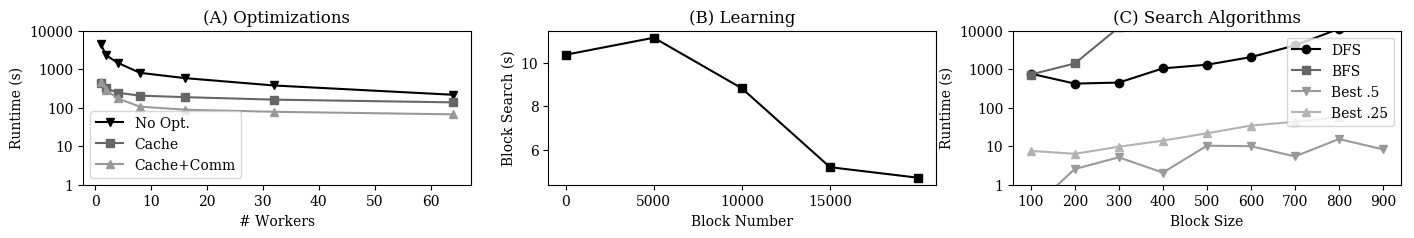
\includegraphics[width=\textwidth]{exp/exp6.png}
 \caption{\small 
   (A) Both the materialization (Cache) and distributed communication (Comm) optimizations contribute to improved scale-out runtimes.
   (B) The learned pruning rules improve the search costs for each subsequent block-wise partition.  
   (C) Best-first search is better than BFS and DFS; reducing $\gamma$ prunes more candidates at the expense of lower accuracy.   \ewu{Make sure to update the label for Best-First 2 and 4 to Gamma=0.5 and Gamma=0.25} \ewu{Fix all y-axes}
 \label{fig:opt}}
\end{figure*}
